\documentclass[paper=letter, fontsize=11pt]{scrartcl}
\usepackage{comment}
\usepackage{graphicx}
\usepackage[T1]{fontenc}
\usepackage{fourier}
\usepackage[english]{babel}
\usepackage{amsmath,amsfonts,amsthm}
\usepackage{acronym}
\usepackage{listings}
\usepackage{sectsty}
\usepackage{fancyhdr}
\pagestyle{fancyplain}
\allsectionsfont{\centering \normalfont\scshape}
\fancyhead{}
\fancyfoot[L]{}
\fancyfoot[C]{}
\fancyfoot[R]{\thepage}
\renewcommand{\headrulewidth}{0pt}
\renewcommand{\footrulewidth}{0pt}
\setlength{\headheight}{13.6pt}
\numberwithin{equation}{section}
\numberwithin{figure}{section}
\numberwithin{table}{section}
\setlength\parindent{0pt}
\newcommand{\horrule}[1]{\rule{\linewidth}{#1}}

\title{	
\normalfont \normalsize 
\textsc{University of Victoria, Computer Science Department} \\ [25pt]
\horrule{0.5pt} \\[0.4cm]
\huge CSC-586A Self-Adaptive Systems\
\horrule{2pt} \\[0.5cm]
}

\author{Tory Borsboom, Sean Debroni, Stephan Heinemann}
\date{\normalsize\today}

\begin{document}
\maketitle 

\section{Part III -- Sensor APIs}
\label{part3}

\begin{comment}
iOS
android
arduino
pixhawk / ardupilot / nuttx
- AP\_RangeFinder (maxsonar i$2$c, state object)
- AP\_OpticalFlow (frontend, backend, state object)
- AP\_AHRS (attitude, heading reference system) uses the optflow object
- sensors.pde uses the optical flow state to supply the EKF and the logger
(update\_opticalflow) - Log.pde writes log messages about the current optical flow state
windows fsx sdk (real hardware interface) -> garmin sdk
- sensors.pde uses the sonar sensor to determine the sonar height (read\_sonar)
- log.pde logs sonar sensor in control\_tuning and optical flow in
log\_write\_optflow
- GCS\_Common.cpp sends the mavlink message to the GCS and uses the sonar height
above ground level (HAGL) - data is used directly and changing logged data is
not effective (mavlink\_msg\_optical\_flow\_send)
- TODO: order longer Iris legs
\end{comment}

\subsection{Apple iOS Gyroscope API}
\label{ios_gyroscope_api}
\par

\subsection{Android Magnetic Compass API}
\label{androis_compass_api}

\subsection{NuttX / ArduPilot PX4 Optical Flow and Sonar API}
\label{ardupilot_flow_api}
\par
The {\em ArduPilot}\footnote{http://ardupilot.com/} autopilot stack supports a
wide range of sensors to be used with any of the supported vehicle types
including {\em Plane}, {\em Copter} and {\em Rover}. It builds on top of the
{\em NuttX}\footnote{http://nuttx.org/} operating system and requires the
applicable firmware for the underlying hardware such as the
{\em Pixhawk}\footnote{https://pixhawk.org}.

\par
The supported sensor types include those to capture data about the vehicle's
{\em environment} as well as those related to its own {\em capabilities} in
order to establish an adequate {\em situational awareness}.

\par
Examples of supported environment sensors gather {\em inertial} (attitude and
acceleration), {\em barometric} (altitude and airspeed), {\em magnetic}
(direction), {\em range} (distance), {\em optical} (orientation and recognition)
and {\em satellite} (position) data. Sensors that capture the vehicle's
capability state include a {\em battery monitor} (power consumption and
endurance) and a {\em performance monitor} (scheduler latency). Environment
sensors themselves may provide {\em health} and {\em quality} monitoring
fuctions. Furthermore, all information that is provided by the {\em NuttX}
operating system about its {\em Pixhawk} platform including the available
{\em memory} and {\em filesystem} space can be instrumented to enhance the
vehicle's capability state.

\par
The {ArduPilot} \ac{API} separates sensor {\em frontends} (interfaces) from
their actual {\em backends} (implementation) in order to easily support
different sensors of the same type. These and other \ac{HAL} modules can be
found in the {\verb libraries }
directory\footnote{https://github.com/diydrones/ardupilot} and are, hence,
separate from any concrete vehicle-related software. The {\em Copter} vehicle
employs the sensor \ac{API} through its {\verb sensors.pde } arduino sketch
file which represents an even higher level
\ac{API}\footnote{http://www.arduino.cc/en/pmwiki.php?n=Reference/HomePage}
to the actual vehicle functions such as different autoflight modes.

\par
As a representative example, the structure of the {\em PX$4$ Optical Flow /
Sonar}\footnote{https://pixhawk.org/modules/px4flow} sensor interface shall be
explained. This sensor allows to capture the optical flow, that is, the rate of
translational and rotational changes in a captured image, in order to establish
positional information. The optical flow camera is mounted on the bottom of the
{\em Iris}\footnote{http://3drobotics.com/iris/} quadcopter body pointing
downwards and sampling the floor pattern that is being overflown. Since the
aircraft can be tilted (pitch and bank) and flown at different altitudes, a
range finder (sonar sensor) on the same sensor board is employed to relate the
optical flow information to the measured ground distances accordingly. Assuming
the actual attitude of the aircraft based on inertial sensors, an actual ground
distance can be derived from the sonar slant range readings.

\par
Figure \ref{fig:optical_flow_api} shows a small extract of the optical flow
sensor frontend \ac{API} in the {\verb libraries/ } {\verb AP_OpticalFlow }
directory possessing the sensor state data structure as well as methods that determine
flow and body rates in a two-dimensional image. The interface itself
furthermore consists of methods that determine the health of the sensor and the
quality of the data being captured by it.

\begin{figure}[h]
	\begin{lstlisting}
	class OpticalFlow
	{
	    //...
	public:
		//...
	    bool enabled() const { return _enabled; }
	    bool healthy() const { return backend != NULL && _flags.healthy; }
	    void update(void);
	    uint8_t quality() const { return _state.surface_quality; }
	    const Vector2f& flowRate() const { return _state.flowRate; }
	    const Vector2f& bodyRate() const { return _state.bodyRate; }
	    uint8_t device_id() const { return _state.device_id; }
	    uint32_t last_update() const { return _last_update_ms; }
	
	    struct OpticalFlow_state {
	        uint8_t device_id;
	        uint8_t  surface_quality;
	        Vector2f flowRate;
	        Vector2f bodyRate;
	    };
	private:
		//...
	};
	\end{lstlisting}
	\caption{Optical Flow Sensor \ac{API}}
	\label{fig:optical_flow_api}
\end{figure}

\par
Figure \ref{fig:range_finder_api} shows an \ac{API} extract of the range finder
component of the optical flow sensor board. On the {\em PX$4$ Optical Flow}
board, a sonar sensor is employed to obtain range in order to relate optical
flow to ground distance. This concrete implementation is abstracted by the
more generic range finder \ac{API} in the %{\verb libraries/AP_RangeFinder }
directory.

\begin{figure}[h]
	\begin{lstlisting}
	class RangeFinder
	{
	public:
		//...
	    struct RangeFinder_State {
	        uint8_t                		instance;
	        uint16_t               		distance_cm;
	        uint16_t               		voltage_mv;
	        enum RangeFinder_Status		status;
	        uint8_t                		range_valid_count;
			//...
	    };
	    //...
	    void update(void);
	    uint16_t distance_cm() //...
	    int16_t ground_clearance_cm() //...
	    RangeFinder_Status status(void) //...
	    bool has_data() //...
	    uint8_t range_valid_count() //...
	private:
		//...
	};
	\end{lstlisting}
	\caption{Range Finder \ac{API}}
	\label{fig:range_finder_api}
\end{figure}

\par
The {\verb sensors.pde } arduino sketch file uses the above \ac{API} in order
to provide the {\em Copter} vehicle with necessary sensor data to perform its
functions such as automatic flight modes. The overall static structure is shown
in Figure \ref{fig:of_sensor_board_api}.

\begin{figure}[h]
	\centering
    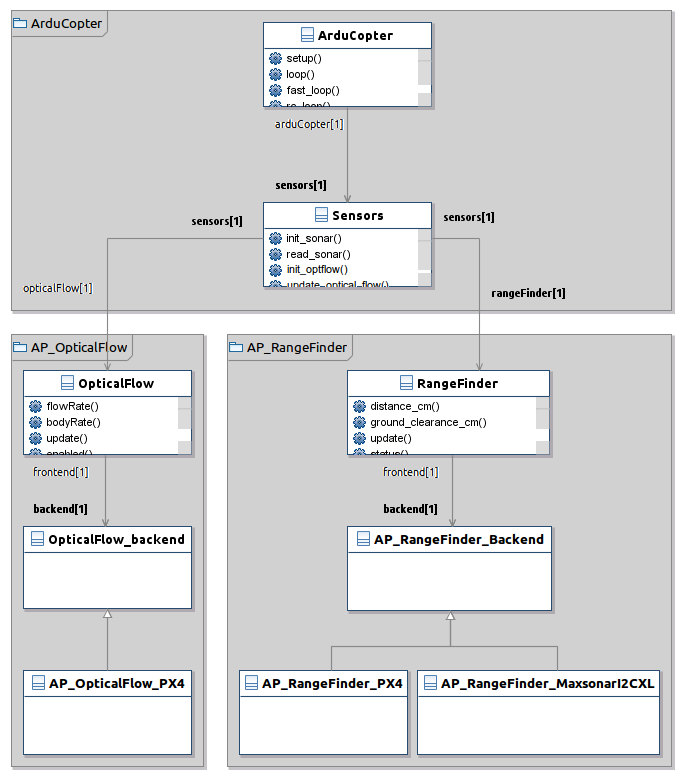
\includegraphics[width=400px]{graphics/OpticalFlowDiagram.png}
	\caption{PX4 Optical Flow Sensor Board \ac{API}}
	\label{fig:of_sensor_board_api}
\end{figure}

\clearpage
\label{appendix}
\section{Figures}
\label{figures}

\begin{figure}[h]
	\centering
    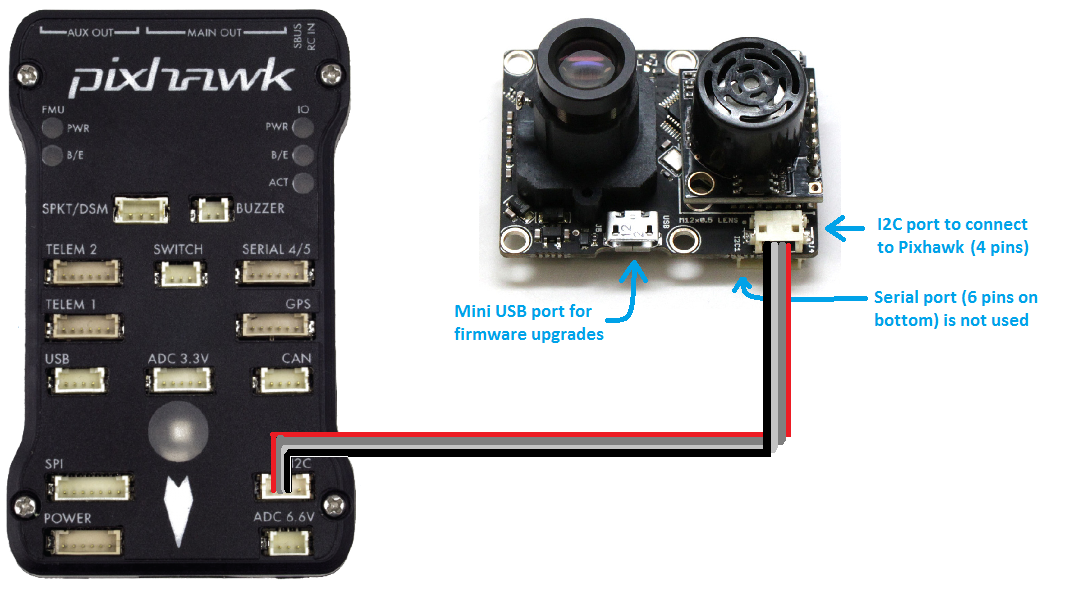
\includegraphics[width=300px]{graphics/PixhawkPX4Flow.png}
	\caption{Pixhawk PX4 Flow Connection}
	\label{fig:pixhawk_px4_flow_connection}
\end{figure}

\begin{figure}[h]
	\begin{lstlisting}[basicstyle=\scriptsize]
class OpticalFlow { //...
public: //...
	bool enabled() const { return _enabled; }
	bool healthy() const { return backend != NULL && _flags.healthy; }
	uint8_t quality() const { return _state.surface_quality; }
	const Vector2f& flowRate() const { return _state.flowRate; }
	const Vector2f& bodyRate() const { return _state.bodyRate; }
	uint8_t device_id() const { return _state.device_id; }
    //...
    struct OpticalFlow_state {
    	uint8_t device_id;
    	uint8_t  surface_quality;
    	Vector2f flowRate;
    	Vector2f bodyRate;
    };
private: //...
};
	\end{lstlisting}
	\caption{Optical Flow Sensor \ac{API}}
	\label{fig:optical_flow_api}
\end{figure}

\begin{figure}[h]
	\begin{lstlisting}[basicstyle=\scriptsize]
class RangeFinder {
public: //...
	enum RangeFinder_Status {
		RangeFinder_NotConnected = 0,
		RangeFinder_NoData,
		RangeFinder_OutOfRangeLow,
		RangeFinder_OutOfRangeHigh,
		RangeFinder_Good
	};
	
	struct RangeFinder_State {
		uint8_t instance;
		uint16_t distance_cm;
		uint16_t voltage_mv;
		enum RangeFinder_Status status;
		uint8_t range_valid_count;
		bool pre_arm_check;
		uint16_t pre_arm_distance_min;
		uint16_t pre_arm_distance_max;
	};
	//...
	uint16_t distance_cm() const { return distance_cm(primary_instance); }
	uint16_t voltage_mv() const { return voltage_mv(primary_instance); }
	int16_t ground_clearance_cm() const { return _ground_clearance_cm[primary_instance]; }
	RangeFinder_Status status(void) const { return status(primary_instance);
	//...
private: //...
};
	\end{lstlisting}
	\caption{Range Finder \ac{API}}
	\label{fig:range_finder_api}
\end{figure}

\begin{figure}[h]
	\centering
    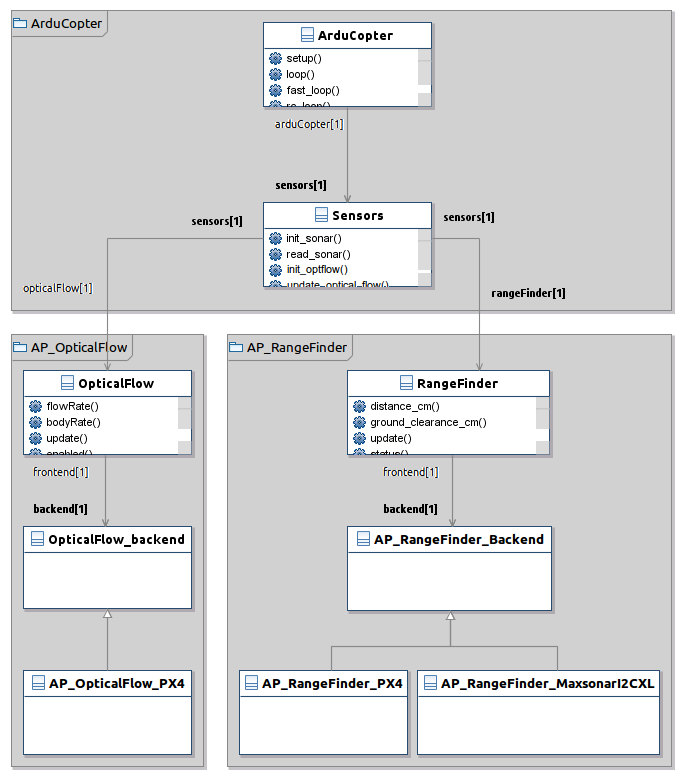
\includegraphics[width=400px]{graphics/OpticalFlowDiagram.png}
	\caption{PX4 Optical Flow Sensor Board \ac{API}}
	\label{fig:of_sensor_board_api}
\end{figure}

\begin{figure}[h]
	\begin{lstlisting}[basicstyle=\scriptsize]
static void stabilize_run()
{
    //...
    // in the stabilizing flight mode check the current flight envelope
    // measured by the optical flow sensor
    checkEnvelope();
    //...
}

#define BODY_RATE_ENVELOPE 4.0f
#define FLOW_RATE_ENVELOPE 1.0f
#define MAX_ALT 1.0f

static bool checkBodyRateEnvelope() {
        Vector2f bodyRate = optflow.bodyRate();
        return ((bodyRate.x > -BODY_RATE_ENVELOPE) && (bodyRate.y < BODY_RATE_ENVELOPE));
}

static bool checkFlowRateEnvelope() {
        Vector2f flowRate = optflow.flowRate();
        return ((flowRate.x > -FLOW_RATE_ENVELOPE) && (flowRate.y < FLOW_RATE_ENVELOPE));
}

static bool checkAltitudeEnvelope() {
        float hagl = 0.0f;
        ahrs.get_NavEKF().getHAGL(hagl);
        return (hagl <= MAX_ALT);
}

static void checkEnvelope() {
        // if the flight envelope is violated, then notify an envelope alert
        // notification subscribers include the tone alert and LED
        if (!checkBodyRateEnvelope() || !checkFlowRateEnvelope() || !checkAltitudeEnvelope()) {
                hal.console->printf("envelope violated\n");
                AP_Notify::flags.envelope_alert = true;
        } else {
                hal.console->printf("envelope satisfied\n");
                AP_Notify::flags.envelope_alert = false;
        }
}
	\end{lstlisting}
	\caption{Application Snippets}
	\label{fig:application_snippets}
\end{figure}

\clearpage
\section{Acronyms}
\label{acronyms}

\begin{acronym}
	\acro{AHRS}{Attitude and Heading Reference System}\\
		An attitude and heading reference system consists of sensors on
		three axes that provide attitude information for aircraft, including
		heading, pitch and yaw.They are designed to replace traditional
		mechanical gyroscopic flight instruments and provide superior
		reliability and accuracy.
		\footnote{http://en.wikipedia.org/wiki/Attitude\_and\_heading\_reference\_system}
	\acro{API}{Application Programming Interface}\\
		In computer programming, an application programming interface is a set
		of routines, protocols, and tools for building software applications.
		An API expresses a software component in terms of its operations,
		inputs, outputs, and underlying types. An API defines functionalities
		that are independent of their respective implementations, which allows
		definitions and implementations to vary without compromising each
		other.
		\footnote{http://en.wikipedia.org/wiki/Application\_programming\_interface}
	\acro{CPS}{Cyber-Physical System}\\
		A cyber-physical system is a system of collaborating computational
		elements controlling physical entities. Today, a precursor generation
		of cyber-physical systems can be found in areas as diverse as
		aerospace, automotive, chemical processes, civil infrastructure,
		energy, healthcare, manufacturing, transportation, entertainment, and
		consumer appliances.
		\footnote{http://en.wikipedia.org/wiki/Cyber-physical\_system}
	\acro{HAL}{Hardware Abstraction Layer}\\
		Hardware abstractions are sets of routines in software that emulate
		some platform-specific details, giving programs direct access to the
		hardware resources.
		\footnote{http://en.wikipedia.org/wiki/Hardware\_abstraction}
	\acro{II}{Industrial Internet}\\
		The Industrial Internet refers to the integration of complex physical
		machinery with networked sensors and software.
		\footnote{http://en.wikipedia.org/wiki/Industrial\_Internet}
	\acro{IIoT}{Industrial Internet of Things}\\
		The Industrial Internet of Things is a subdiscipline of the \acs{IoT},
		which describes IP-enabled systems in factories, offices and other
		commercial (and sometimes government) facilities. It is the part of the
		\acs{IoT} that focuses on how smart machines, networked sensors and
		sensor analytics can help improve business-to-business initiatives
		across a wide variety of industries, especially manufacturing.
		\footnote{http://itlaw.wikia.com/wiki/Industrial\_Internet\_of\_Things}
	\acro{IoT}{Internet of Things}\\
		The Internet of Things is the network of physical objects or "things"
		embedded with electronics, software, sensors and connectivity to enable
		it to achieve greater value and service by exchanging data with the
		manufacturer, operator and/or other connected devices.
		\footnote{http://en.wikipedia.org/wiki/Internet\_of\_Things}
	\acro{LED}{Light-Emitting Diode}
		A light-emitting diode is a two-lead semiconductor light source. It is
		a pn-junction diode, which emits light when activated. When a suitable
		voltage is applied to the leads, electrons are able to recombine with
		electron holes within the device, releasing energy in the form of
		photons.
		\footnote{http://en.wikipedia.org/wiki/Light-emitting\_diode}
	\acro{SoSs}{System of Systems}\\
		System of systems is a collection of task-oriented or dedicated systems
		that pool their resources and capabilities together to create a new,
		more complex system which offers more functionality and performance
		than simply the sum of the constituent systems.
		\footnote{http://en.wikipedia.org/wiki/System\_of\_systems}
	\acro{ToE}{Theory of Everything}\\
		A theory of everything or final theory, ultimate theory, or master
		theory is a hypothetical single, all-encompassing, coherent theoretical
		framework of physics that fully explains and links together all
		physical aspects of the universe.
		\footnote{http://en.wikipedia.org/wiki/Theory\_of\_everything}
	\acro{UAV}{Unmanned Aerial Vehicle}\\
		An unmanned aerial vehicle, known in the mainstream as a drone and also
		referred to as an unpiloted aerial vehicle and a remotely piloted
		aircraft by the International Civil Aviation Organization, is an
		aircraft without a human pilot aboard.
		\footnote{http://en.wikipedia.org/wiki/Unmanned\_aerial\_vehicle}
	\acro{ULSS}{Ulta-Large-Scale System}\\
		Ultra-large-scale system is a term used in fields including Computer
		Science, Software Engineering and Systems Engineering to refer to
		software intensive systems with unprecedented amounts of hardware,
		lines of source code, numbers of users, and volumes of data.
		\footnote{http://en.wikipedia.org/wiki/Ultra-large-scale\_systems}
\end{acronym}

\clearpage
\label{bibliography}
\bibliographystyle{plain}
\bibliography{csc-586a-13}

\end{document}
